\documentclass{article}
\usepackage{setspace}
\usepackage[T1]{fontenc}
\usepackage[utf8]{inputenc}
\usepackage[a4paper,top=3.5cm,left=3cm,right=3cm,bottom=2.5cm]{geometry}
\usepackage[brazil]{babel}
\usepackage{graphicx}
\usepackage{hyperref}
\usepackage{fancyhdr}
\usepackage{background}
\usepackage[a4paper,top=3.5cm,left=3cm,right=3cm,bottom=2.5cm]{geometry}
\usepackage{lmodern}
\usepackage{tikz}
\usepackage[font={small,stretch=0.80,it}]{caption}

%Configurando o mapa mental
\usetikzlibrary{mindmap}

%Configurando a path das imagens
\graphicspath{{../../imagens/capitulo1/}}

%Configurando a imagem de background
\backgroundsetup{
scale=1,
angle=0,
opacity=0.4,
contents={%
  
\includegraphics[width=\paperwidth,height=\paperheight]{wallpaper.png}
  }%
}

%configurando os hyperlinks
\hypersetup{
    colorlinks=true,
    linkcolor=blue,
    filecolor=magenta,      
    urlcolor=cyan,
}

%configurando os headers
\pagestyle{fancy}
\fancyhf{}
\rhead{LDO}
\lhead{Capítulo 1}
\rfoot{Página \thepage}

%configurando identação e separação de parágrafos
\parindent 1.27cm
\parskip   6pt

%títulos,autor e data
\title{\textbf{Capítulo 1 \\ Um pouco sobre Machine Learning}}
\author{Thiago Henriques Nogueira}
\date{Novembro de 2020}

\begin{document}
    
    %Inserindo o título
    \maketitle
   
    \begin{center}
        \begin{tikzpicture}[mindmap, grow cyclic, every node/.style=concept, concept color=orange!40,
        level 1/.append style={level distance=5cm,sibling angle=90},
        level 2/.append style={level distance=3cm,sibling angle=45}]

        \node{Um pouco sobre Machine Learning}
            child [concept color=blue!30] { node {Inicio \\ \ref{sec:introduction}}
                child { node {\href{https://www.sas.com/pt_br/insights/analytics/deep-learning.html}{Deep Learning}}}
                child { node {\href{https://openai.com/}{Open AI}}}
                child { node {\href{https://debuild.co/}{debuild.co}}}
            }
            child [concept color=yellow!30] { node {Development \\ \ref{sec:desenvolvimento}}
                child { node {\href{https://rockcontent.com/br/blog/algoritmo-do-youtube/}{Algoritmo de pesquisa}}}
                child { node {\href{https://youtu.be/oWcVTWLgACM}{Tags}}}
                child { node {\href{https://super.abril.com.br/tecnologia/como-funciona-a-recomendacao-de-videos-do-youtube/}{Recomen dação}}}
            };
            % child [concept color=teal!40] { node {Amazon \\ \ref{sec:amazon}}
            %     child { node {\href{https://www.noticiastecnologia.com.br/amazon-ajusta-algoritmo-de-pesquisa-para-priorizar-os-proprios-produtos}{Relevância ou Lucro?}}}
            %     child { node {\href{https://www.visualcapitalist.com/amazon-worlds-most-valuable-retailer/}{Maior varejista dos EUA}}}
            % }
            % child [concept color=purple!50] { node {Deep Blue \\ \ref{sec:deep_blue}}
            %     child { node {\href{https://pt.wikipedia.org/wiki/Garry_Kasparov}{Garry Kasparov}}}
            %     child { node {\href{https://pt.wikipedia.org/wiki/IBM}{IBM}}}
            %     child { node {\href{https://canaltech.com.br/produtos/o-que-e-supercomputador/}{Super computador}}}
            % };
        \end{tikzpicture}

    \end{center}


    %Aumentando o tamanho padrão das fontes
    \Large
    
    %Iniciando a seção 'Inicio'
    \section{Início} \label{sec:introduction}

    Antes de entrarmos no assunto precisamos saber: o que Machine Learning significa? Bom traduzindo ao 
    pé da letra, Machine Learning está ligado ao Aprendizado de Máquina. Porém por mais que esse 
    assunto tenha aparecido mais durante a atualidade, seu termo foi criado a muito tempo atrás.

    Em 1959 \href{https://en.wikipedia.org/wiki/Arthur_Samuel}{Arthur Samuel}, conhecido como o 
    pioneiro da inteligência artificial, utilizou o termo Machine Learning pela primeira vez. 

    \begin{figure}[htp]
        \centering
        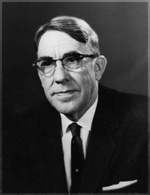
\includegraphics[scale=1.5]{ArthurSamuel.jpg}
        \caption{\href{https://youtu.be/pbVwH8o837A}{Imagem de Arthur Samuel}}
    \end{figure}

    Nessa época, ele trabalhava em um algoritmo capaz de jogar xadrez, que devido a um sistema de
    pontuação, melhorava suas estratégias gradativamente após cada partida. O programa foi nomeado
    Games of Checkers.

    %Forçar o programa ir para uma nova página
    \newpage
    \section{Desenvolvimento} \label{sec:desenvolvimento}

    \begin{figure}[htp]
        \centering
        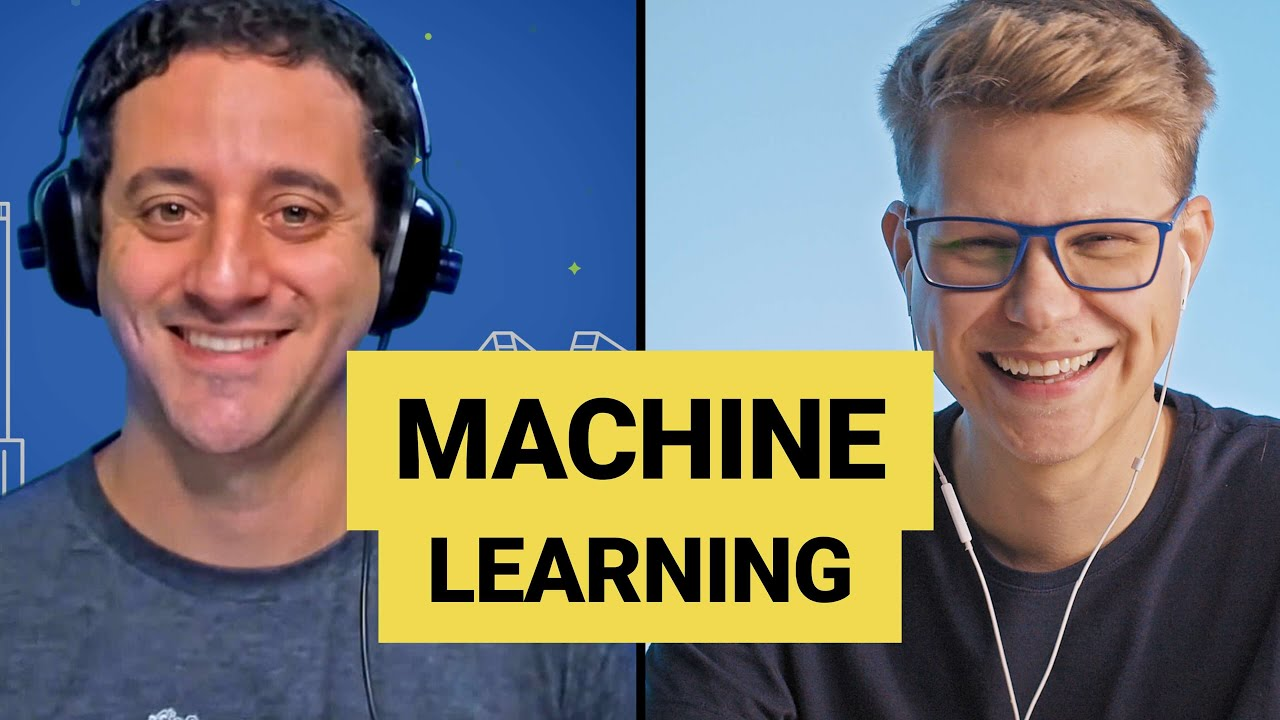
\includegraphics[scale=0.3]{maxresdefault.jpg}
        \caption{\href{https://youtu.be/pbVwH8o837Ahttps://www.youtube.com/watch?v=JyGGMyR3x5I}{Machine Learning: Tutorial prático usando apenas o navegador (é sensacional!!!)}}
    \end{figure}


    Se você não assistiu esse vídeo do canal do Filipe Deschamps, é uma ótima oportunidade para 
    quem quer aprender sobre essa área. Juntamente com o co-fundador da Alura, Guilherme Silveira, 
    eles desenvolvem e demonstram conceitos básicos tudo através do navegador.

    Agora que o conceito de Machine Learning foi estabelecido, resta saber como ela funciona. De 
    um jeito bem simples, a maior parte dos algoritmos com o passar do tempo, começam a criar e 
    aprimorar suas redes neurais com base nos obstáculos e falhas consecutivas de se obter o 
    resultado desejado. 
    
    Entre as redes neurais podemos observar os perceptrons, considerados os tipos mais simples de 
    rede neural. Inventada em 1958 por \href{https://en.wikipedia.org/wiki/Arthur_Samuel}{Frank Rosenblatt}, 
    os perceptrons são representações dos neurônios do algoritmo.  

    \newpage
    \section*{\centering Material extra}\label{sec:extra} %Criando uma tag para que possa ser referência em outras partes do programa

    %Iniciando listagem
    \begin{itemize}
        \item \href{https://www.youtube.com/watch?v=Iuz_jc96bQk}{O que é Machine Learning? Hipsters Ponto Tube}
        \item \href{https://www.youtube.com/watch?v=HcqpanDadyQ}{O que é aprendizado de maquina(AI Adventures)}
        \item \href{https://www.zdnet.com/article/what-is-machine-learning-everything-you-need-to-know/}{What is machine learning? Everything you need to know}
        \item \href{https://www.sbc.org.br/images/flippingbook/computacaobrasil/computa_39/pdf/CompBrasil_39_180.pdf}{Revista da Sociedade Brasileira de Computação}
    \end{itemize}

    \newpage

    %Iniciando referências
    \begin{thebibliography}{3}
        \bibitem{frank} 
        Frank Rosenblatt \\
        \href{http://www.csis.pace.edu/~ctappert/srd/b1.pdf}{The Father of Deep Learning} 
        
        \bibitem{arthur} 
        Arthur Samuel \\
        \href{https://cs.stanford.edu/memoriam/professor-arthur-samuel}{Stanford  File} 
    
        \bibitem{arthur2} 
        Arthur Samuel pt.2 \\
        \href{https://history-computer.com/ModernComputer/thinkers/Samuel.html}{History Computer} 
    \end{thebibliography}
    
\end{document}